\documentclass{article}

% Definitions
\newcommand{\pavo}{{\tt pavo}}  % you can use \pavo{} to print pavo as package
\newcommand{\code}[1]{{\tt #1}}  % way to plot out code
\setlength{\parindent}{0in}
\setlength{\parskip}{.1in}
\setlength{\textwidth}{140mm}
\setlength{\oddsidemargin}{10mm}
\usepackage{amsmath}
\usepackage{hyperref}

\usepackage{Sweave}
\begin{document}

\Sconcordance{concordance:pavo.tex:pavo.rnw:%
1 12 1 1 0 3 1 1 7 80 1 1 2 4 0 1 2 15 1}



\title{\pavo{}: {\bf P}erceptual {\bf A}nalysis, {\bf V}isualization and {\bf O}rganization of Color Data in R}
\author{Rafael Maia, Paul-Pierre Bitton, Chad Eliason}

\maketitle

\section*{Introduction}

\pavo{} is an R package developed with the goal of establishing a flexible and integrated 
workflow for working with spectral color data. It includes functions that take advantage of
new data classes in order to work seamlessly from importing raw data to visualization and 
analysis.

Although \pavo{} deals largely with spectral reflectance data from bird feathers, it is meant 
to be applicable for a range of taxa and applications. It provides flexible ways to input
spectral data from a variety of equipment manufacturers, process these data, extract variables 
and produce publication-quality graphics.

This is a random edit by Rafael.

\pavo{} was written with the following workflow in mind:

% numbered list of things
\begin{enumerate}
\item {\bf O}rganize spectral data by inputting files, processing spectra (e.g., to remove
noise, negative values, smooth curves, etc.)
\item {\bf A}nalyze the resulting files, either using typical tristimulus color variables (hue,
saturation, brightness) or using visual models based on perceptual data from the taxon of interest.
\item {\bf V}isualize the output
\end{enumerate}

Below we will show the main functions in the package in an example workflow. 

\section{Data Description}

The data used in this example is available from 
\href{https://github.com/rmaia/pavo/blob/master/vignette_data/vignette_data.zip}{github by clicking here}. 
You can download and extract it to follow the vignette.

The data consists of reflectance spectra obtained using Avantes equipment and software from 
seven bird species: Northern Cardinal (\emph{Cardinalis cardinalis}), Wattled Jacana (\emph{Jaca
na jacana}), Baltimore Oriole (\emph{Icterus galbula}), Peach-fronted Parakeet (\emph{Aratinga 
aurea}), American Robin (\emph{Turdus migratorius}), Violet-green Swallow (\emph{Tachycineta 
thalassina}), and Sayaca Tanager (\emph{Thraupis sayaca}). Several individuals were measured 
(sample size varies by species), and 3 spectra were collected from each individual.

The samples do not have the same sample sizes and have additional peculiarities that should 
emphasize the flexibility \pavo{} offers, as we'll see below.

\section{Organizing and Processing Spectral Data}

\subsection{Importing Data}

The first thing we need to do is import the spectral data into R using the funciton 
\code{getspec()}. Since the spectra were obtained using Avantes software, we will need to 
specify that the files have the "\code{.ttt}" extension. Further, the data is organized in 
subdirectories for each species. \code{getspec} does recursive sampling, and may include the 
names of the subdirectories in the spectra name if desired. A final issue with the data is that 
it was collected using a computer with international numbering input, which means it uses commas 
instead of periods as a decimal separator. We can specify that in the function call.

I have downloaded the file and placed it in a directory called 
"\nolinkurl{/github/pavo/vignette_data}". By default, \code{getspec} will search for files in 
the default folder, but a different one can be specified:

\begin{Schunk}
\begin{Sinput}
> specs <- getspec("~/github/pavo/vignette_data/", ext="ttt", decimal=",", 
+                  subdir=T, subdir.names=F)
> specs[1:10,1:4]
\end{Sinput}
\begin{Soutput}
    wl cardinal.0001 cardinal.0002 cardinal.0003
1  300        5.7453        8.0612        8.0723
2  301        6.0181        8.3926        8.8669
3  302        5.9820        8.8280        9.0680
4  303        6.2916        8.7621        8.7877
5  304        6.6277        8.6819        9.3450
6  305        6.3347        9.6016        9.4834
7  306        6.3189        9.5712        9.3533
8  307        6.7951        9.4650        9.9492
9  308        7.0758        9.4677        9.8587
10 309        7.2126       10.6172       10.5396
\end{Soutput}
\begin{Sinput}
> dim(specs) #data has 235 spectra, from 300 to 700 nm
\end{Sinput}
\begin{Soutput}
[1] 401 235
\end{Soutput}
\end{Schunk}

When \pavo{} imports spectra, it creates an object of class \code{rspec}, which inherits attributes from the \code{data.frame} class:
\begin{Schunk}
\begin{Sinput}
> is.rspec(specs)
\end{Sinput}
\begin{Soutput}
[1] TRUE
\end{Soutput}
\end{Schunk}

If you already have multiple spectra in a single data frame that you'd like to use with \pavo{} 
functions, you can use the command \code{as.rspec} to convert it to an rspec object. The 
function will attempt to identify the wavelength variable or, if it doesn't have one, it can be 
specified in the function call.

\subsection{Processing Data}

\subsection{Averaging Spectra}

As previously described, our data constitutes of multiple individuals, and each was measured 
three times, as is common in order to avoid measurement bias. A good way to visualize the 
repeatability of our measurements is to plot the spectra of each individual separately. The 
function \code{explorespec} provides an easy way of doing so. You may specify the number of 
spectra to be plotted in the same panel using the argument \code{specreps}, and the function 
will adjust the number of panels per page accordingly. We will exemplify this function using 
only 10 of the cardinal individuals measured:

\begin{Schunk}
\begin{Sinput}
> explorespec(specs[,1:40], specreps=3) 
> # 39 spectra plus the first (wl) column
\end{Sinput}
\end{Schunk}

\begin{figure} % h=here, t=top, b=bottom, p=floating page
\begin{center}
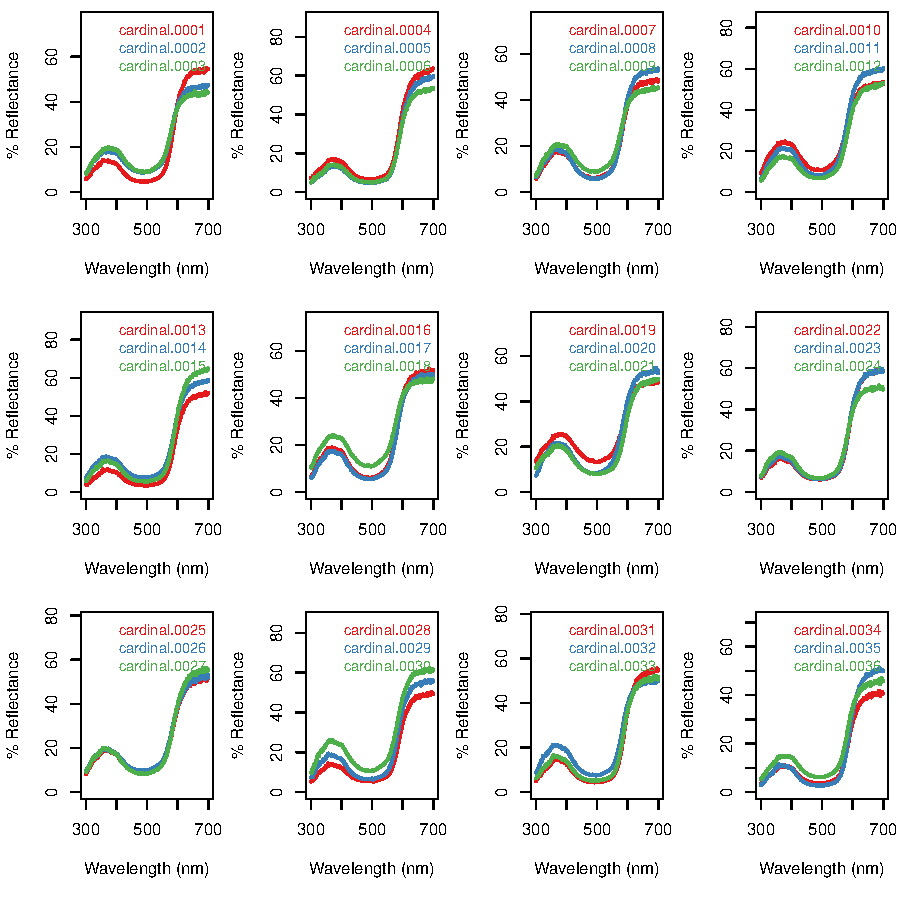
\includegraphics[width=6in]{pavo-explorespecfig}
\end{center}
\caption{Result from \code{explorespec}, showing the three measurements for each individual in separate panels}
\label{fig1}
\end{figure}

\clearpage{}

So our first step would be to take the average of each of these three measurements in order to 
obtain average individual spectra to be used in further analyses. The function \code{aggspec} 
does this. The \code{by} argument can be either a number (specifying how many specs should be 
averaged for each new sample) or a vector specifying the identities of the spectra to be 
combined (see below):

\begin{Schunk}
\begin{Sinput}
> mspecs <- aggspec(specs, by=3, FXN=mean)
> mspecs[1:5, 1:4]
\end{Sinput}
\begin{Soutput}
   wl cardinal.0001 cardinal.0004 cardinal.0007
1 300      7.292933      5.676700      6.387233
2 301      7.759200      5.806700      6.698200
3 302      7.959333      5.858467      6.910500
4 303      7.947133      6.130267      7.357567
5 304      8.218200      6.127933      7.195267
\end{Soutput}
\begin{Sinput}
> dim(mspecs) #data now has 79 spectra, one for each individual
\end{Sinput}
\begin{Soutput}
[1] 401  79
\end{Soutput}
\end{Schunk}

Now we'll use the \code{aggspec} function again, but this time to take the average spectrum for 
each species. However, each species has a different number of samples, so we can't use the 
\code{by} argument as before. Instead we will use regular expressions to create a species name 
vector by removing the numbers that identify individual spectra:

\begin{Schunk}
\begin{Sinput}
> # create a vector with species identity names
> spp <- gsub('\\.[0-9].*$','',names(mspecs))[-1]
> table(spp)
\end{Sinput}
\begin{Soutput}
spp
cardinal   jacana   oriole parakeet    robin  swallow 
      12        9        9       13       10        7 
 tanager 
      18 
\end{Soutput}
\end{Schunk}

Instead, we are going to use the \code{spp} vector we created to tell the \code{aggspec} 
function how to average the spectra in \code{mspec}:

\begin{Schunk}
\begin{Sinput}
> sppspec <- aggspec(mspecs, by=spp, FXN=mean)
> sppspec[1:5, ]
\end{Sinput}
\begin{Soutput}
   wl cardinal   jacana   oriole parakeet    robin  swallow
1 300 7.049397 7.334781 3.889693 7.629954 3.981747 4.035262
2 301 7.254161 7.354033 3.905322 7.746882 3.914297 4.036576
3 302 7.444275 7.452556 4.126619 7.886877 4.187073 4.098371
4 303 7.820686 8.085541 4.390685 8.491367 4.507410 4.132943
5 304 7.843394 7.714526 4.183637 8.658000 4.068800 4.026381
    tanager
1  9.021043
2  9.525854
3  9.405980
4 10.199843
5  9.684522
\end{Soutput}
\begin{Sinput}
> explorespec(sppspec, 7)
\end{Sinput}
\end{Schunk}

\begin{figure}[h] % h=here, t=top, b=bottom, p=floating page
\begin{center}
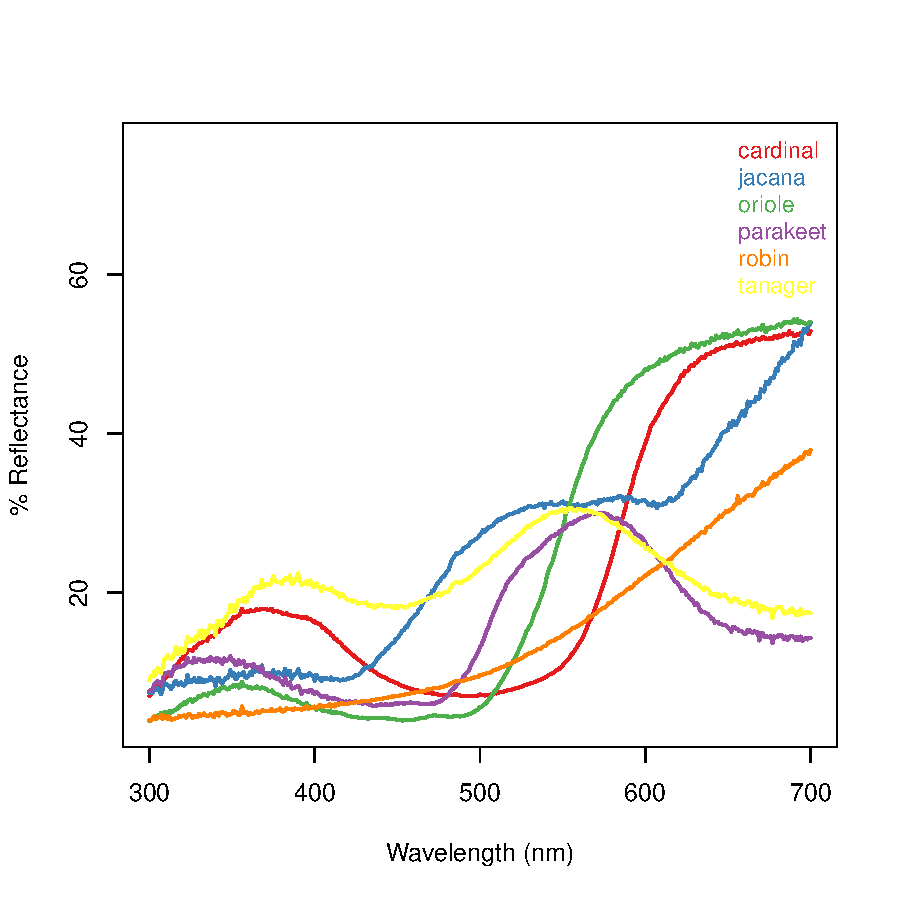
\includegraphics[width=4in]{pavo-exploresppmeans}
\end{center}
\caption{Result from \code{explorespec} for species means}
\label{fig2}
\end{figure}

\section{Analyzing Spectral Data}

\subsection{Overview}

add description here

\subsection{Variables calculated}

% A table for filling in Montgomerie's color variables
\begin{table}[h]
\begin{center}
\begin{tabular}{l l l} \hline
{\bf Color} & \\
{\bf Variable} & {\bf Equation} & {\bf Description} \\ 
\hline
\code{B1} & {$\sum_{\lambda={300}}^{700} R_\lambda$} & \parbox[t]{3in}{Total brightness, total reflectance}  \\
\code{B2} & {$B_\text{1}/n_\text{wl}$} & \parbox[t]{3in}{Mean brightness.} \\
\code{B3} & {$R_\text{max}$} & \parbox[t]{3in}{Intensity.} \\
\code{S1} & {} & \parbox[t]{3in}{Chroma, spectral purity.} \\
\code{S2} & {$R_\text{max}/R_\text{min}$} & \parbox[t]{3in}{Spectral saturation} \\
\code{S3} & {} & \parbox[t]{3in}{} \\
\code{S4} & {} & \parbox[t]{3in}{} \\
\code{S5} & {} & \parbox[t]{3in}{} \\
\code{S6} & {} & \parbox[t]{3in}{} \\
\code{S7} & {} & \parbox[t]{3in}{} \\
\code{S8} & {} & \parbox[t]{3in}{} \\
\code{S9} & {} & \parbox[t]{3in}{} \\
\code{S10} & {} & \parbox[t]{3in}{} \\
\code{H1} & {$\lambda_\text{Rmax}$} & \parbox[t]{3in}{Hue: wavelength of peak reflectance} \\
\code{H2} & {} & \parbox[t]{3in}{} \\
\code{H3} & {} & \parbox[t]{3in}{} \\
\code{H4} & {} & \parbox[t]{3in}{} \\
\code{H5} & {} & \parbox[t]{3in}{} \\
\hline
\end{tabular}
\end{center}
\caption{\label{table:tristim}
The complete set of tristimulus variables calculated by \code{summary} in \pavo{}}
\end{table}

Color variables described in Table \ref{table:tristim}.

blah blah blah\footnote{some footnote text here} and also this.

\section{Visualizing Spectral Data}

<<<<<<< HEAD
\begin{Schunk}
\begin{Sinput}
> data(sicalis)
> plot(sicalis, type='o', col=spec2rgb(sicalis))
> #plot(sicalis, type='s', col=spec2rgb(sicalis))
\end{Sinput}
\end{Schunk}

\begin{figure} % h=here, t=top, b=bottom, p=floating page
\begin{center}
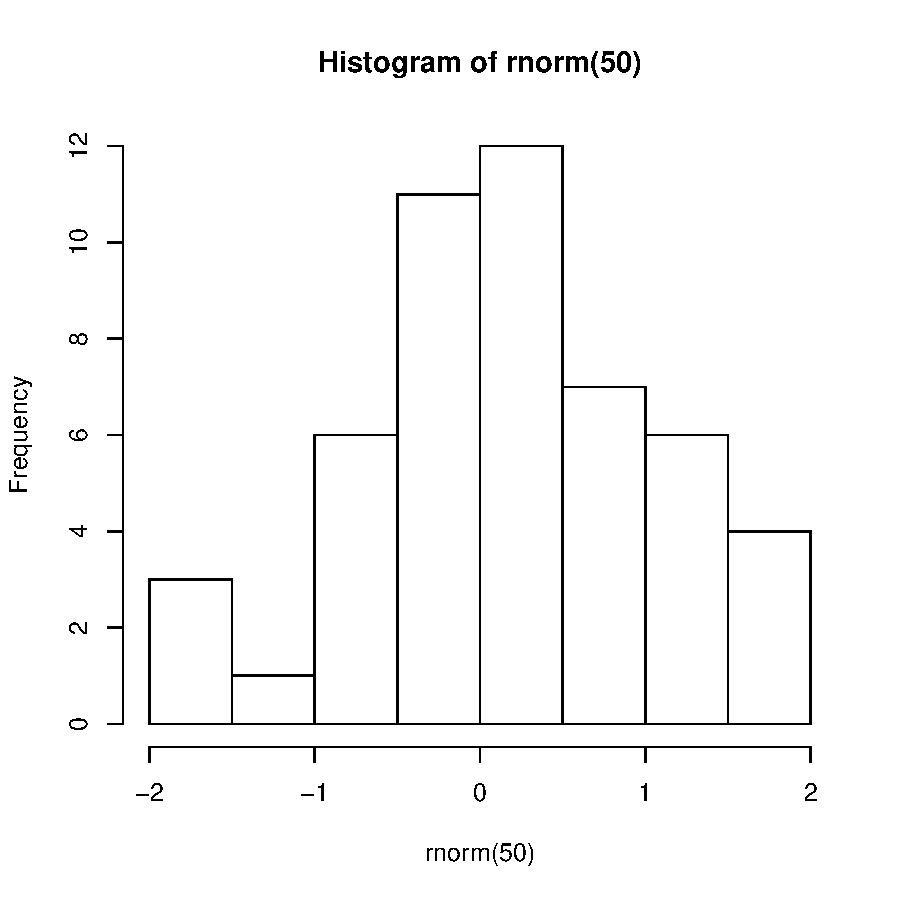
\includegraphics[width=3in]{pavo-fig1}
\end{center}
\caption{Sample plot.}
\label{fig1}
\end{figure}

=======
This is how you plot something ...
>>>>>>> 410ed83d33665cdb62e17e176f63f0d3ce6a4bae

\begin{figure} % h=here, t=top, b=bottom, p=floating page
\begin{center}
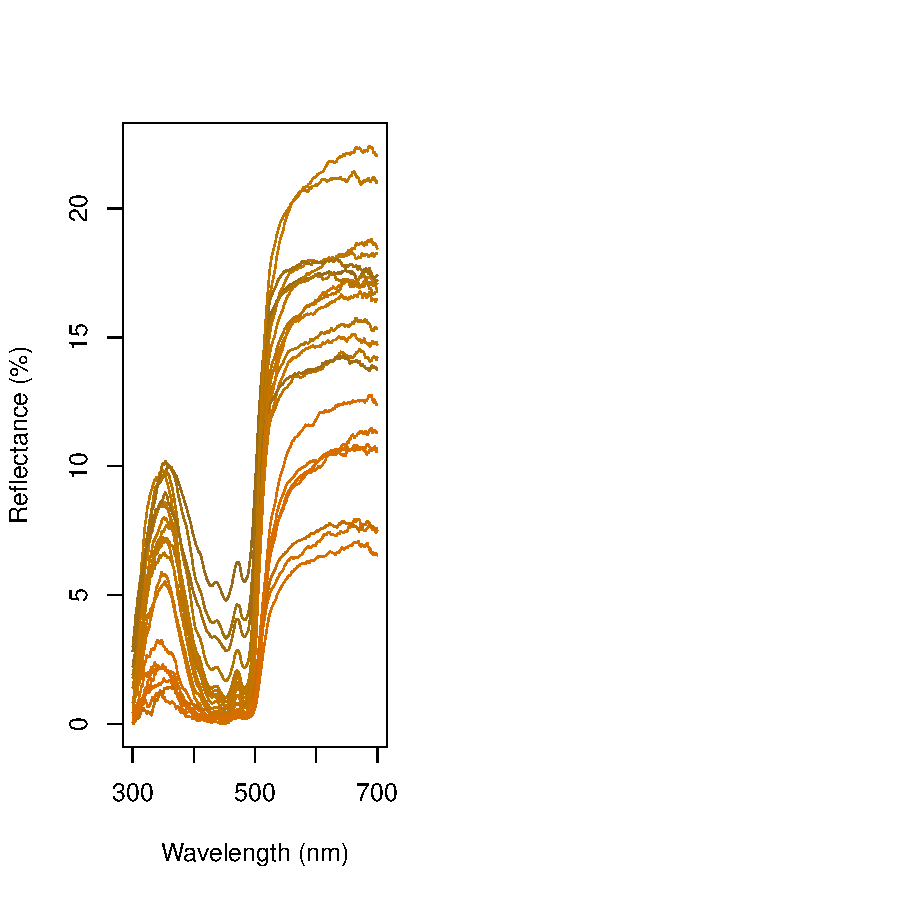
\includegraphics[width=4in, height=3in]{pavo-overlay}
\end{center}
\caption{Overlay plot with colors calculated from human color matching functions}
\label{figure:overlay}
\end{figure}

Colors can be mapped to spectra using \code{spec2rgb} as shown in 
Figure \ref{figure:overlay}.

\section*{Examples}


\begin{Schunk}
\begin{Sinput}
> hist(rnorm(50))
\end{Sinput}
\end{Schunk}

<<<<<<< HEAD
=======
%\begin{figure}[h] % h=here, t=top, b=bottom, p=floating page
%\begin{center}
%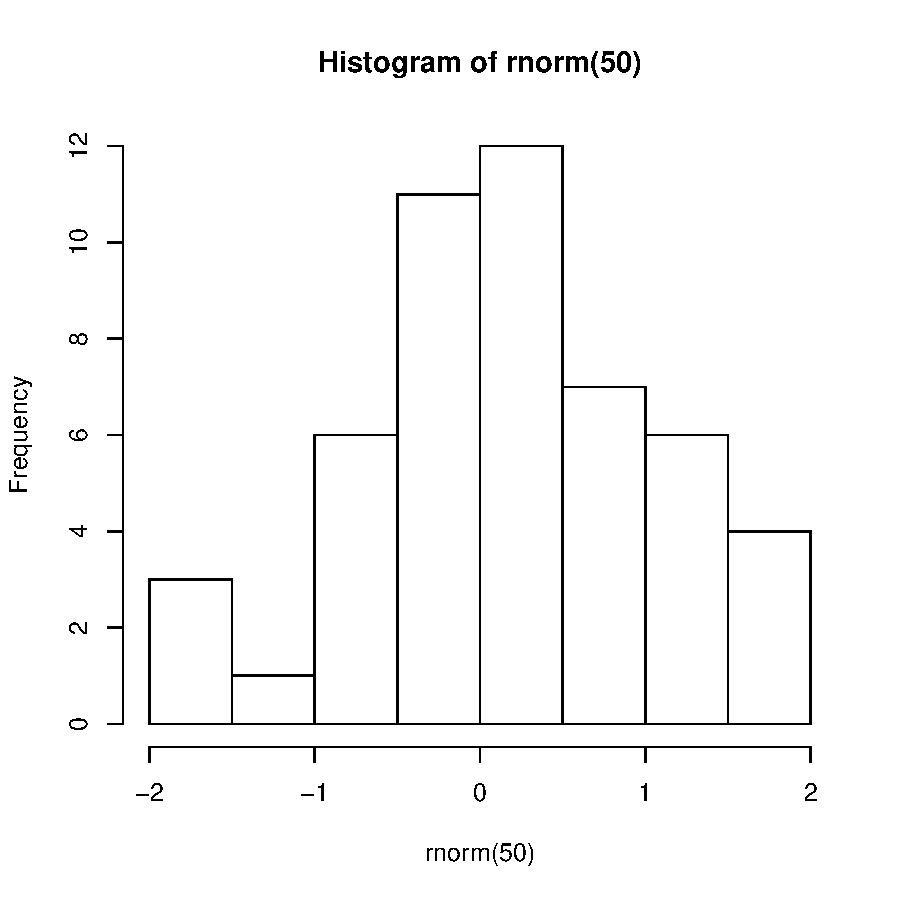
\includegraphics[width=5in]{pavo-fig1}
%\end{center}
%\caption{Sample plot.}
%\label{fig1}
%\end{figure}
>>>>>>> 410ed83d33665cdb62e17e176f63f0d3ce6a4bae

\subsection*{More examples}

Some more examples:

\bibliography{}

\end{document}
